\section{EMPIRICAL EVALUATION}
\label{sec:results}
In this section, we evaluate the performance of our system using real-world event streams provided by the datAcron project in the context of maritime domains. The used event streams describe trajectory critical points (i.e., synopses) of moving vessels, which are derived from raw AIS messages as was  described in \cite{synopses1}. In particular, for our evaluation we used a data set of synopses contains $4,684,444$ critical points of $5055$ vessels sailing in the Atlantic Ocean during the period from 1 October 2015 to 31 March 2016. We use it to generate a simulated stream of event tuples  \textit{(id,type,timestamp, longitude, latitude, annotation, speed, heading)},    where $type$ $\in \Sigma$ and $\Sigma=$ $\{$\textit{VerySlow ,Slow, Moving, Sailing, Stopping} $\}$ that is based on the  vessel speed, and $annotation$ is an attribute to encode the trajectory movement events such as speed change, slow motion, and gap in reporting. In our experiments, we monitor a pattern $\mathcal{P}=Sailing$ that detects when the vessel under way (sailing).


\subsubsection*{Experimental setup} We ran our experiments on single-node standalone Flink cluster deployed on a server (Ubuntu 17.04) with Intel(R) Core(TM) i7-7700 CPU @ 3.60GHz X 8 processors and 32GB RAM. We used Apache Flink v1.3.2 and Apache Kafka v0.10.2.1 for our tests.


\subsubsection*{Evaluation criteria} Our goal is to evaluate our distributed pattern prediction based on enabling the synchronization of PMC models between the predictors against the isolated ones (i.e., without exchanging information), we compare the predictive performance in terms of :
\begin{enumerate*}[label=(\roman*)]
	
\item  average $\mathit{precision = \frac{\#\ of\ correct\ predictions}{\#\ of\ total\ predictions}}$ per predictor node

\item $\mathit{cumulative\ error}$ that presents the aggregated number of all wrong predictions.

\item $\mathit{recall}$ is the fraction of the pattern's full matches are successfully predicted by the system at least once. 

\end{enumerate*} 
Moreover, we study the communication cost by measuring the $\mathit{cumulative\ communication}$ that captures the number of  synchronization related messages, which is introduced by employing the static or dynamic synchronization schemes of the distributed online learning protocol. In next, we present the experimental results for the for the pattern  $\mathcal{P}=Sailing$ with $m=2$, batch size $b=100$,  variance threshold $\Delta=2$, and PMC prediction threshold $\theta_{fc}=80\%$.

\begin{figure}[]
	
	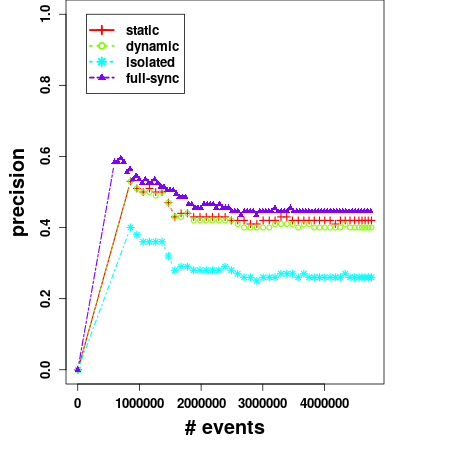
\includegraphics[width=.5\textwidth]{figures/precision.png}
	
	\caption{Precision scores.}
	\label{fig:precsions}
\end{figure}

\subsubsection*{Experimental results} Figure ~\ref{fig:precsions} depicts the precision scores (i.e., average precision of prediction model per vessel)  of all approaches, namely, isolated without synchronization, continuous synchronization, static (periodic), and our proposed approach based on the dynamic synchronization scheme. While Figure ~\ref{fig:error} shows the average cumulative error per predictor.       


\begin{figure}[]
	
	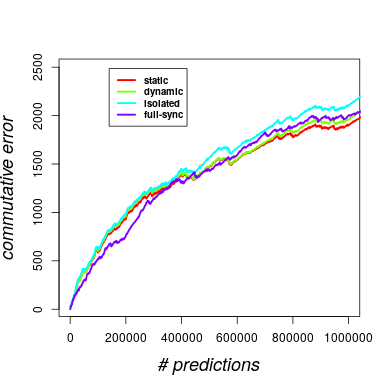
\includegraphics[width=.5\textwidth]{figures/error.png}
	
\caption{Commutative error.}
\label{fig:error}
\end{figure}

\par In Table ~\ref{tab:recall}, we present the statistics of recall results for the different approaches. It can be seen 


\begin{figure}[]
	
	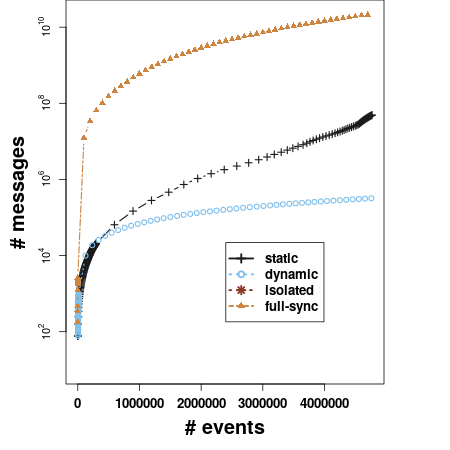
\includegraphics[width=.5\textwidth]{figures/communication.png}
	
	\caption{Commutative communication.}
	\label{fig:comm}
\end{figure}
\begin{table}[]
	\caption{Recall results.}
	\label{tab:recall}
	\begin{tabular}{lll}
		\toprule
		Approach &Mean&Max\\
		\midrule
		isolated & 0.1948  & 0.23 \\
		static & 0.1976  &  0.23 \\
		dynamic & 0.1974  & 0.23 \\
		full-sync & 0.1979  & 0.33 \\
		\bottomrule
	\end{tabular}
\end{table}


Figure ~\ref{fig:comm} provides the accumulated communication required for the three approaches based on the distributed online learning. As expected, larger amount of communication is required for the continuous synchronization comparing to static and dynamic approaches, and it can bee seen with small variance threshold $\Delta=2$ that we can reduce the communication using the dynamic synchronization and comparing the (static) periodic method, and furthermore, still preserving the predictive performance as was shown in Figures ~\ref{fig:precsions} and ~\ref{fig:error}.  
